\documentclass{article}

% Formatting
\usepackage[utf8]{inputenc}
\usepackage[margin=1in]{geometry}
\usepackage[titletoc,title]{appendix}
\usepackage{graphicx,float}
\usepackage{minted}
\usemintedstyle{borland}
\usepackage{biblatex}
\addbibresource{references.bib}

% Title content
\title{Tipología y Ciclo de vida de los datos: Web Scraping}
\author{Ismael Rosende Rey y Chantal López Procopio}
\date{Noviembre, 2020}

\begin{document}

\maketitle

% Resumen
\begin{abstract}
    En  el  presente  proyecto,  hemos creado un  web  crawler  capaz  de  navegar  por  la  web  del supermercado Carrefour, extrayendo los  datos  de los diferentes  productos que allí se exponen y sus atributos principales (precios,  ofertas  y promociones). Este ejercicio tiene como finalidad entender y poner en práctica los conceptos aprendidos  en la  asignatura  de Tipología  y  Ciclo  de  Vida  de  los  Datos, asignatura perteneciente al Máster en Ciencia de los Datos de la Universitat Oberta de Catalunya, para  realizar  un Web Scraping.
\end{abstract}

% Título Dataset
\section{Título Dataset}
El título escogido para este dataset es CarrefourDailyPricing, ya que guarda relación directa con el propósito de la araña que hemos creado para este proyecto, ella se explica detalladamente a continuación.

%  Descripción Dataset
\section{Descripción del Dataset}
El dataset CarrefourDailyPricing está formado por una lista con los productos del supermercado Carrefour, guardando los datos más importantes como: la categoría del producto, su precio actual, precio por kilogramo, ofertas y promociones.

% Representación gráfica
\section{Gráfica}

\begin{figure}[H]
    \centering
    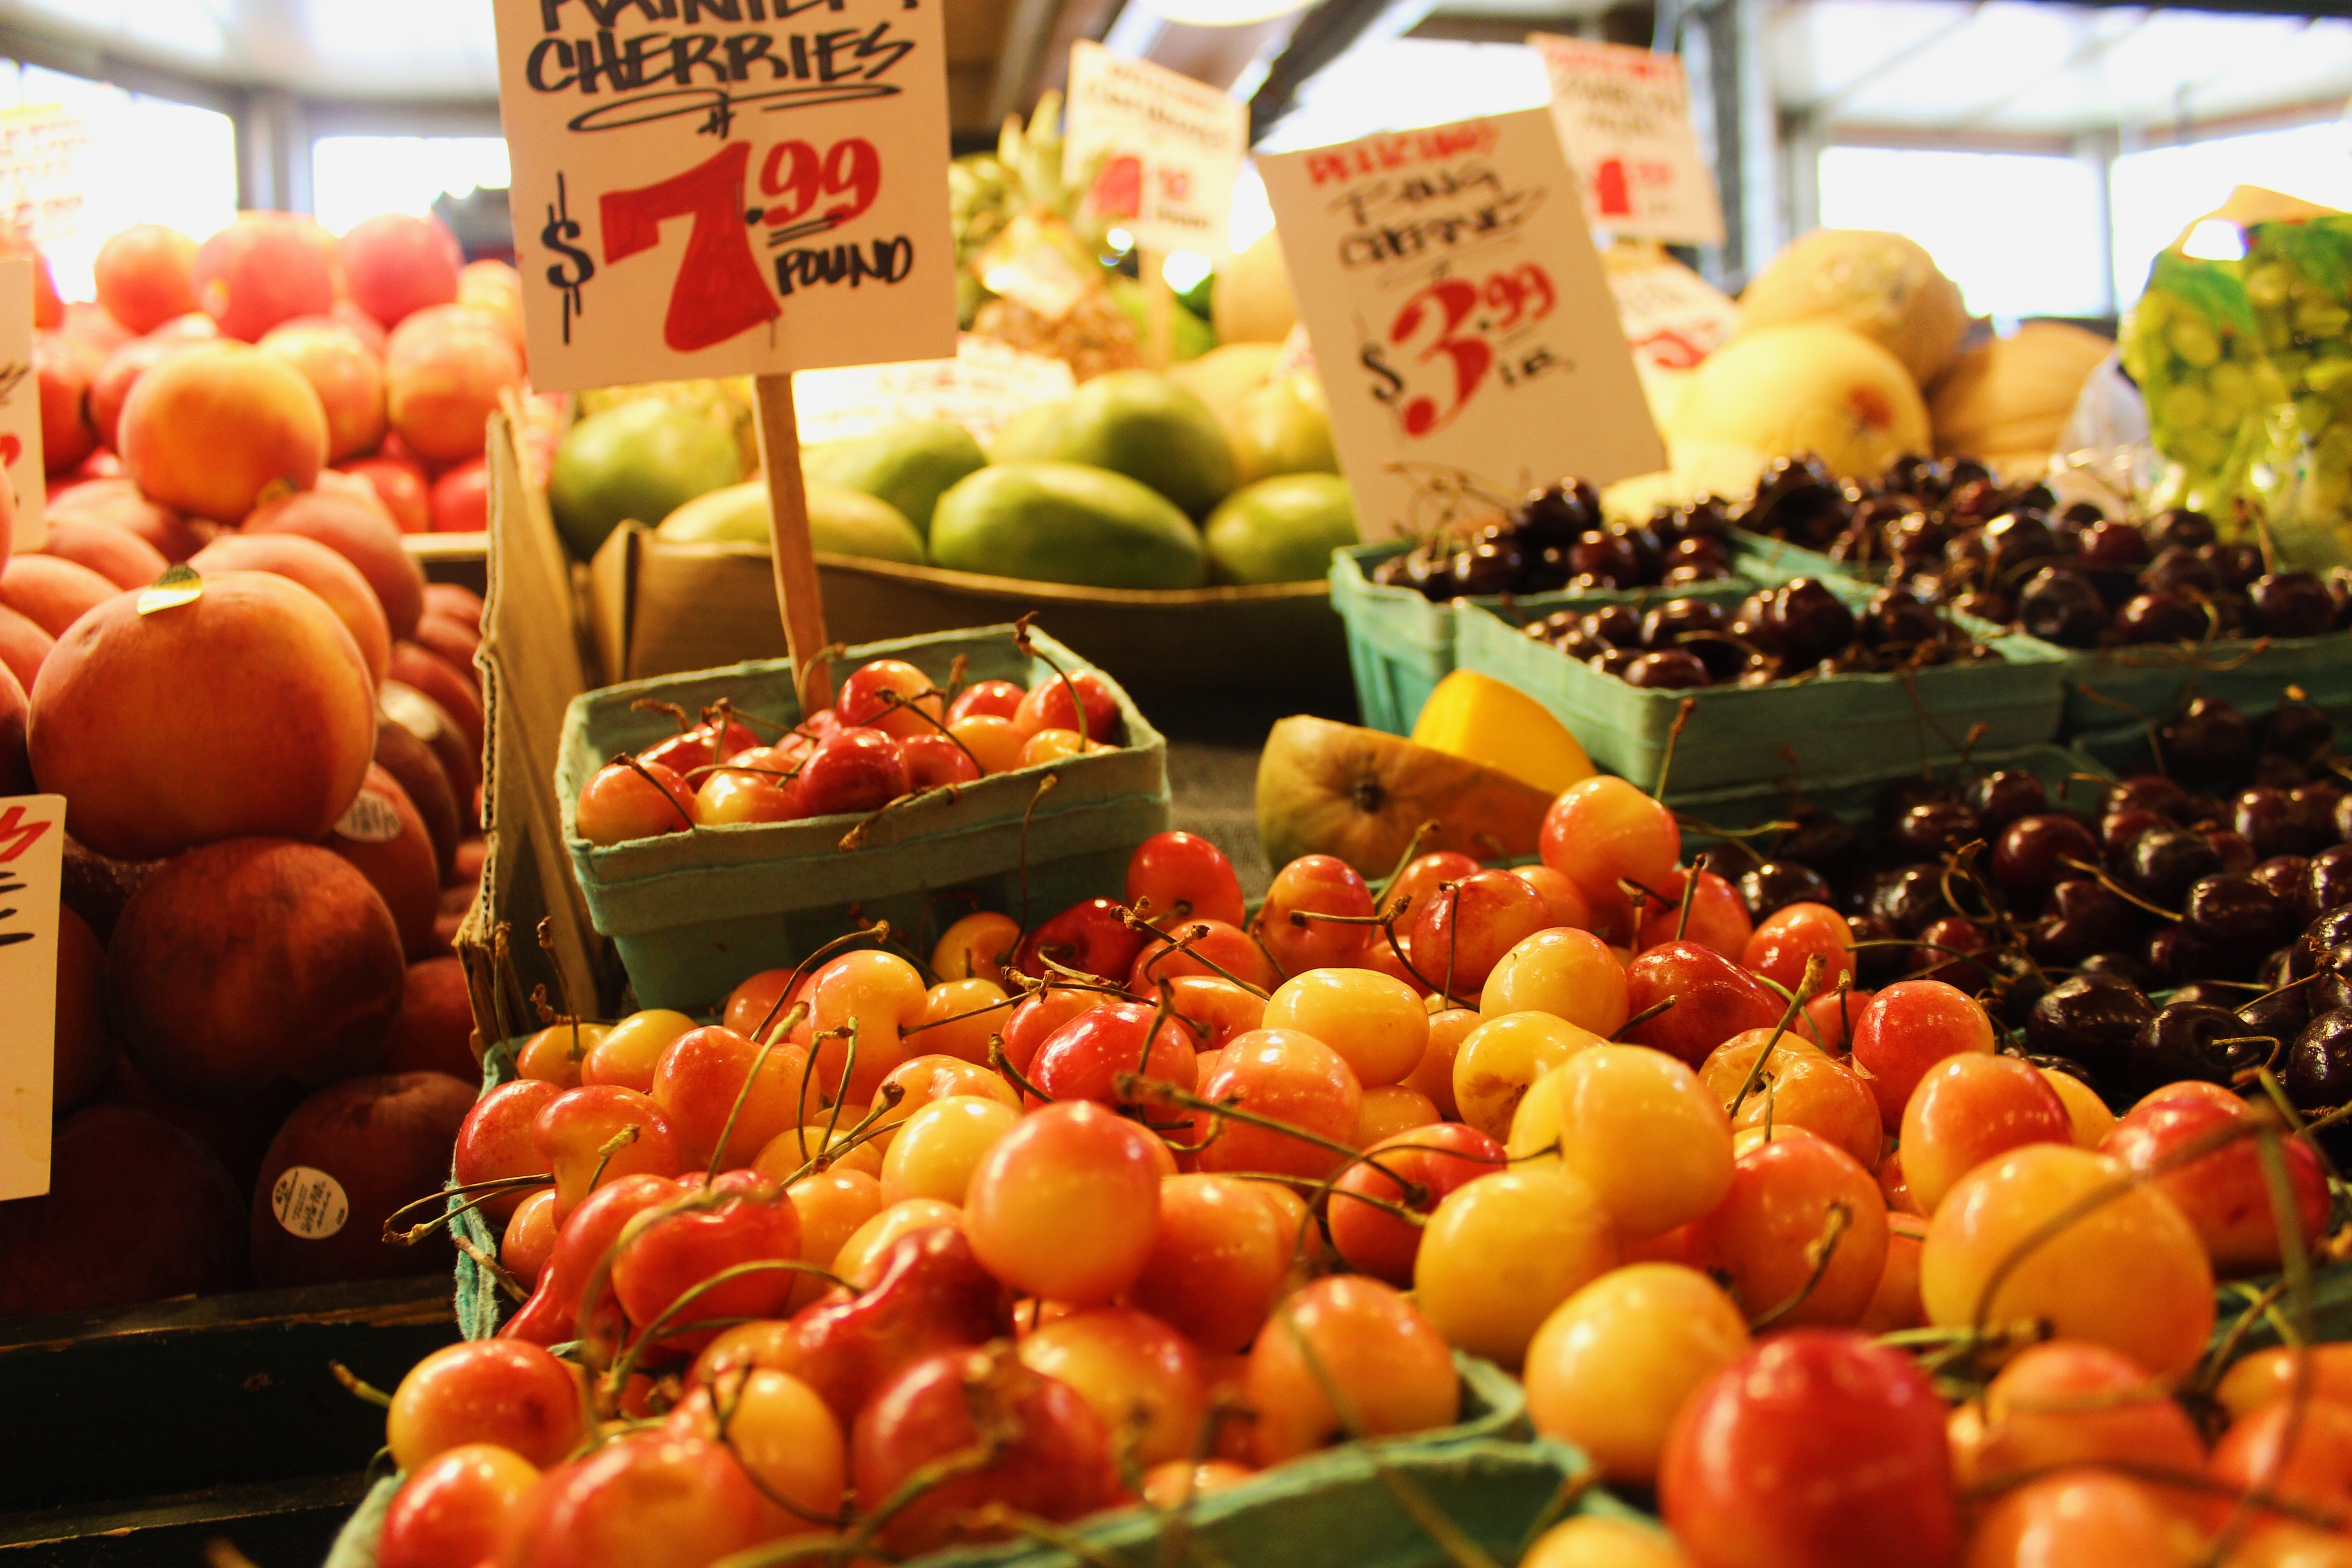
\includegraphics[width=0.4\linewidth]{super.jpg}
    \caption{Esquema del Dataset}
    \label{fig:dubs}
\end{figure}

\pagebreak
% Contenido del Dataset
\section{Contenido del dataset}
El dataset CarrefourDailyPricing contiene los siguientes atributos:

\begin{itemize}
    \item {Categoría}: Sección del supermercado a la que pertenece un producto.
    \item {Descripción}: Nombre que tiene asociado elproducto en el supermercado.
    \item {Precio}: Precio de venta actual.
    \item {Precio/Kg}: Precio por cada kilogramo
    \item {previo}: Precio anterior a la oferta.
    \item {Precio oferta}: Precio de venta durante la oferta.
    \item {Promociones}: Promociones activas para cada producto.
    \item {Enlace}: Enlace donde se puede encontrar el producto en cuestión.
\end{itemize}

La araña está programada para actualizar el dataset una vez al día, a las 8:00hrs, generando un csv nuevo cogiendo los atributos ya mencionados.

% Agradecimientos
\section{Agradecimientos}
Para  elaborar  este, recurrimos a  la  web  de Carrefour  para  extraer  los  datos  de  los productos que el supermercado ofrece dentro de su oferta comercial. Agradecemos por su aporte a este proyecto como  nuestra  fuente  principal de  datos,  pero  también haber sido de gran ayuda durante nuestra  formación  y aprendizaje.

% Inspiración
\section{Inspiración}
Este conjunto de datos busca recoger diariamente información de interés sobre cada producto en  el  supermercado Carrefour.  Durante la  elaboración  de  este  proyecto,  no  solo  buscamos  la extracción de datos, sino también poder llevar un registro donde comparar las subidas y bajadas de precios en un período de tiempo determinado. Por esa razón, hemos programado la araña para que recorra la web diariamente, y así poder remarcar los productos en oferta, cada cuánto tiempo  ocurren  y  su  evolución  en  el  tiempo.  También,  serviría  para  estudiar  el  impacto  que tienen sobre la economía las crisis como la que vivimos actualmente del covid.

% Licencia
\section{Licencia}
El dataset CarrefourDailyPricing tendrá una licencia del tipo Attribution-NonCommercial-ShareAlike 4.0. Lo que implica que las personas son libres de utilizar el dataset como prefieran, pero sin obtener una retribución de tipo comercial. La creación del dataset fue hecho meramente con fines educativos, por lo que nuestro principal interés recae en que otras personas puedan aprender de él, modificarlo a gusto y ampliar su contenido como les parezca conveniente dentro de estos parámetros.

\pagebreak
% Código dataset
\section{Código del Dataset}
El código fuente y el dataset generado con nuestro script “carrefourScraping”, se pueden encontrar en el siguiente enlace: https://github.com/equipoUOC/CarrefourTracker

% Contribuciones al proyecto
\section{Contribuciones}

\begin{table}[H]
    \centering
    \begin{tabular}{rll}
    & Contribuciones & Firma \\
    \hline
    & Investigación previa & IRR, CLP  \\
    & Redacción de las respuestas & IRR, CLP \\
    & Desarrollo código & IRR, CLP \\
    \end{tabular}
\end{table}


% Recursos
\section{Recursos}
\begin{itemize}
    \item Subirats, L., Calvo, M. (2018). Web Scraping. Editorial UOC.
    \item SLawson, R. (2015). Web Scraping with Python. Packt Publishing Ltd. Chapter 2.Scraping the Data.

\end{itemize}

\end{document}
